% ****** Start of file .tex ******
%
%   This file is based on apssamp.tex, part of the APS files in the REVTeX 4.1 distribution.
%   Version 4.1r of REVTeX, August 2010
%
%   Copyright (c) 2009, 2010 The American Physical Society.
%   Samuel Balula, Pedro Ribeiro, Luís Macedo, Eduardo Neto 2013
%   See the REVTeX 4 README file for restrictions and more information.
%
% TeX'ing this file requires that you have AMS-LaTeX 2.0 installed
% as well as the rest of the prerequisites for REVTeX 4.1
%
% See the REVTeX 4 README file
% It also requires running BibTeX. The commands are as follows:
%
%  1)  latex filename.tex
%  2)  bibtex filename
%  3)  latex filename.tex
%  4)  latex filename.tex

\documentclass[%
  reprint,
  %superscriptaddress,
  %groupedaddress,
  %unsortedaddress,
  %runinaddress,
  %frontmatterverbose, 
  %preprint,
  %showpacs,preprintnumbers,
  nofootinbib,
  %nobibnotes,
  %bibnotes,
  amsmath,amssymb,
  aps,
  %pra,
  %prb,
  %rmp,
  %prstab,
  %prstper,
  %floatfix,
  10pt,
  a4paper
]{revtex4-1}

\if11
% Usual (decimal) numbering
\renewcommand{\thesection}{\arabic{section}}
\renewcommand{\thesubsection}{\thesection.\arabic{subsection}}
\renewcommand{\thesubsubsection}{\thesubsection.\arabic{subsubsection}}

% Fix references
\makeatletter
\renewcommand{\p@subsection}{}
\renewcommand{\p@subsubsection}{}
\makeatother

\fi

\usepackage{listings}
\usepackage{color}
\usepackage{facil}                      % Pacote pessoal
\usepackage{verbatim}                   % Apresentação de código
\usepackage{graphicx}                   % Include figure files
\usepackage{dcolumn}                    % Align table columns on decimal point
\usepackage{bm}                         % bold math
\usepackage[latin1,utf8]{inputenc}      % Tipos de caracteres
\usepackage[portuges]{babel}            % Português
\usepackage{indentfirst}                % Identação da primeira linha
\usepackage{hyperref}                   % add hypertext capabilities
\usepackage{float}                      %Fixar imagens
 \usepackage{subcaption}
%\usepackage[mathlines]{lineno}          % Enable numbering of text and display math
%\linenumbers\relax                      % Commence numbering lines
%\usepackage[compact]{titlesec}

\usepackage[%showframe,%Uncomment any one of the following lines to test 
%%scale=0.7, marginratio={1:1, 2:3}, ignoreall, % default settings
%%text={7in,10in},centering,
margin=0.5in,        %diminuir margens
%total={6.5in,8.75in}, top=1.2in, left=0.9in, 
includefoot
%height=10in,a5paper,hmargin={3cm,0.8in},
]{geometry}

\begin{document}
%\preprint{APS/123-QED}
%\captionsetup[table]{font=small,skip=0pt}
%\captionsetup[figure]{font=small,skip=0pt}
%\titlespacing{\section}{0pt}{*0}{*0}            %Poupar espaço
%\titlespacing{\subsection}{0pt}{*0}{*0}
%\titlespacing{\subsubsection}{0pt}{*0}{*0}

\lstset{language=Matlab,%
    %basicstyle=\color{red},
	belowcaptionskip=1\baselineskip,
	frame=L,
    breaklines=true,%
    morekeywords={matlab2tikz},
    keywordstyle=\color{blue},%
    morekeywords=[2]{1}, keywordstyle=[2]{\color{black}},
    identifierstyle=\color{black},%
    stringstyle=\color{mylilas},
    commentstyle=\color{mygreen},%
    showstringspaces=false,%without this there will be a symbol in the places where there is a space
    numbers=left,%
    numberstyle={\tiny \color{black}},% size of the numbers
    numbersep=9pt, % this defines how far the numbers are from the text
    emph=[1]{for,end,break},emphstyle=[1]\color{red}, %some words to emphasise
    %emph=[2]{word1,word2}, emphstyle=[2]{style},    
}
% % % % % % % % % % % % % % % % % % % % % % % % % % % % % % % % % % % % % % % % 
%%%%%%%%%%%%%%%%%%%%%%%%%%%%%%%%%% Início %%%%%%%%%%%%%%%%%%%%%%%%%%%%%%%%%%%%%%
% % % % % % % % % % % % % % % % % % % % % % % % % % % % % % % % % % % % % % % %
 

\title{Controlo por retroacção do estado de um braço robot flexível}
\thanks{Relatório do trabalho de laboratório}
\author{Alexandre Aparício}
\email{73252, alexandre.aparicio@tecnico.ulisboa.pt}

\author{Pedro Ribeiro}%
\email{73221, pedro.q.ribeiro@tecnico.ulisboa.pt}
\author{Samuel Balula}%
\email{72735, samuel.balula@tecnico.ulisboa.pt}

\affiliation{
  Instituto Superior Técnico\\
  Mestrado em Engenharia Física Tecnológica\\
  Controlo em Espaço de Estados
}

\collaboration{Grupo 4A de 4ª feira}

\date{\today}

%%%%%%%%%%%%%%%%%%%%%%%%%%%%%%%%%% Abstract %%%%%%%%%%%%%%%%%%%%%%%%%%%%%%%%%%%%
\begin{abstract}
Neste trabalho de laboratório procede-se ao dimensionamento de um controlador por realimentação de variáveis de estado de uma barra flexível actuada por um motor dc, aproximada por um sistema linear, que inclui um observdor assimptótico e seguimento de referência.
O modelo é testado em {\it simulink}, recorrendo tanto a simulações como utilizando o sistema real.
Apresentam-se neste documento os dados experimentais e as respostas às questões laboratoriais.
\end{abstract}
\maketitle


%%%%%%%%%%%%%%%%%%%%%%%%%%%%%%%%%% Introdução %%%%%%%%%%%%%%%%%%%%%%%%%%%%%%%%%%
\section{Controlabilidade}

De acordo com as informações dadas no enunciado, tomando como vector de estado $x$ dado por \eqref{x} as matrizes do modelo de estado linearizado na forma \eqref{lin} são dadas por \eqref{A}, \eqref{B}, \eqref{C}.

\eq[x]{x = \begin{bmatrix}
		x_1 &x_2 &x_3 &x_4 
\end{bmatrix} = \begin{bmatrix}
\theta & \alpha & \dot\theta& \dot\alpha
\end{bmatrix}}

\eq[lin]{\begin{cases}
	\dot x = A x + b u \\
	y = C x
\end{cases}}



\eq[A]{A = \begin{bmatrix}
		0	&0		&1		&0	\\
		0	&0		&0		&1	\\
		0	&566	&-37	&0	\\
		0	&-922	&37		&0	
\end{bmatrix}
}

\eq[B]{b= \begin{bmatrix}
		0 \\
		0\\
		65\\
		-65
\end{bmatrix}}

\eq[C]{c = \begin{bmatrix}
		1 &1	&0	&0
	\end{bmatrix}
}

Pode assim escrever-se a matrix de controlabilidade como \eqref{contr}, calculada em {\it Matlab} como se descreve em \rlis{list1}.

\eq[contr]{\begin{array}{rcl}
		\mathcal{C} &= &
		\begin{bmatrix}
			b &A b & A^2 b & A^3 b
		\end{bmatrix}\\
		&= &
		\begin{bmatrix}
			0         &65       &-2405       &52195 \\
			0         &-65        &2405      &-29055\\
			65       &-2405       &52195     &-569985\\
			-65        &2405      &-29055     &-286195
		\end{bmatrix}
	\end{array}
}

Determinou-se que o sistema é controlável (a dimensão da matriz de controlabilidade é igual ao número de variáveis de estado).

\begin{lstlisting}[label=list1, caption={Código Matlab para o cálculo da matrix de controlabilidade $\mathcal{C}$ e de observabilidade $\mathcal{O}$. As variáveis {\it cntr} e {\it obsr} adquirem valores booleanos, que indicam se o sistema é controlável e/ou observável, respectivamente. As funções {\it controlab} e {\it observab} apresentam-se em anexo em ficheiros com o mesmo nome.}]
[C,cntr]=controlab(A,b);
[O,obsr]=observab(A,c);
\end{lstlisting}


\section{Observabilidade}
A matrix de observabilidade é dada por \eqref{obsr}, calculada em {\it Matlab} como se descreve em \rlis{list1}.


\eq[obsr]{\begin{array}{rcl}
		\mathcal{O} &= &
		\begin{bmatrix}
			c \\
			c A\\
			c A^2\\
			c A^3
		\end{bmatrix}\\
		&= &
		\begin{bmatrix}
			1     &1    &0     &0\\
			0     &0     &1     &1\\
			0  &-356     &0     &0\\
			0     &0     &0  &-356
		\end{bmatrix}
	\end{array}
}
Determinou-se que o sistema é observável (a dimensão da matriz de observabilidade é igual ao número de variáveis de estado).

\section{Diagrama de Bode}
\fig{../img/BodeMalhaAberta.png}{Diagrama de Bode do sistema em cadeira aberta}

Através do diagrama de Bode da \rfig{../img/BodeMalhaAberta.png} é possível concluir que o sistema possui 4 pólos, tal como esperado. O motor DC introduz dois pólos reais\cite{dcmotor} e a barra dois pólos complexos conjugados, característicos de um movimento oscilatório amortecido.

Calcularam-se os valores próprios da matriz A, que correspondem aos pólos do sistema em cadeia aberta, que se apresentam na tabela \ref{tab1}.
Um dos pólos reais está na origem e o restante tem módulo bastante próximo do dos dois pólos complexos conjugados. O efeito destes é assim essencialmente conjunto.
Verifica-se no digrama de Bode que, para cerca de 4Hz dá-se uma variação de fase de -270º devida aos três pólos, que em conjunto com os -90º devidos ao pólo na origem, prefaz a diferença de fase de -360º para grandes valores de frequência. Do mesmo modo, para a amplitude observa-se um declive inicial de -20dB devido ao pólo na origem e um aumento deste em -60dB em cerca de 4Hz, prefazendo um declive de -80dB para grandes valores de frequência.

Tem-se assim que a resposta do sistema se dá para baixas frequências, apresentando atenuações superiores a 60dB para frequências superiores a 10Hz.

\tabela[tab1]{Pólos do sistema em cadeia aberta (valores própios da matriz A)}{ccc}
{
	
$z$	&$\abs{z}$	&$\abs{z}$/(2$\pi$)	\\ 	
rad $s^{-1}$	&rad $s^{-1}$	& Hz \\ \hline
$   0.0000 + 0.0000i$	&$0$	&$0$	\\
$  -7.4016 +23.2085i$	&$24.3601$	&$3.877$	\\
$  -7.4016 -23.2085i$	&$24.3601$	&$3.877$	\\
$ -22.1969 + 0.0000i$	&$22.1969$	&$3.5327$


}

\section{Cálculo do vector de ganhos do controlador e observador}
No cálculo dos ganhos do controlador e observador utilizou-se a função {\it ganhos}, que recebe como argumentos as matrizes de controlabilidade $\mathcal{C}$, observabilidade $\mathcal{O}$ e da dinâmica $A$, e os valores próprios desejados para o controlador e observador, retornando os ganhos calculados com a fórmula de Bass-Gura, conforme se explicita em \rlis{list2}.

Determinaram-se assim os ganhos que se apresentam em \eqref{ganhoK} e \eqref{ganhoL}.
\eq[ganhoK]{
	K = \begin{bmatrix}
	6.0501	&-30.5345	&1.0297	&-0.0933
	\end{bmatrix}
}

\eq[ganhoL]{
	L = 
	\begin{bmatrix}
		33.5\\
		89.5\\
		-1161.2\\
		5088.2
	\end{bmatrix}
	}

\begin{lstlisting}[label=list2, caption={Código Matlab para o cálculo dos ganhos $K$ do controlador e $L$ do observador a partir das matrizes de controlabilidade $\mathcal{C}$, observabilidade $\mathcal{O}$ e da dinâmica $A$, e os valores próprios desejados para o controlador $vpp\_C$ e observador $vpp\_O$. A função {\it ganhos} apresenta-se em anexo no ficheiro com o mesmo nome.}]
[K,L]=ganhos(C,vpp_C,O,vpp_O,A);
\end{lstlisting}
\subsection{Verificação com teorema de separação}
O teorema da separação permite que o controlador e observador sejam dimensionados separamente, já que o polinómio característico do sistema global pode ser escrito como o produto dos polinómios característicos do controlador \eqref{polc} e observador \eqref{polo}.
Realizando numericamente estas expressões obtêm-se os valores próprios, que se verificam corresponder aos requeridos, e que por serem numericamente iguais a estes aqui se omitem.

\eq[polc]{det(sI-A+bK) = 0}
\eq[polo]{det(sI-A+Lc) = 0}


\section{Simulação em {\it simulink}}

Apresenta-se na \rfig{../img/simulink.png} o diagrama da simulação efectuada em {\it simulink}, onde o sistema da esquerda representa o compensador e o da direita o processo. Os parâmetros do compensador apresentam-se em \eqref{compensa} e os do processo em \eqref{processo}.
\eq[compensa]{
	\begin{cases}
		A_c = A - bK - Lc\\
		b_c = -L\\
		C_c = -K\\
		D_c = 0
	\end{cases}
}
\eq[processo]{
	\begin{cases}
		A_p = A\\
		b_p = b\\
		C_p = c\\
		D_p = 0
	\end{cases}
}

\begin{figure*}[t]
  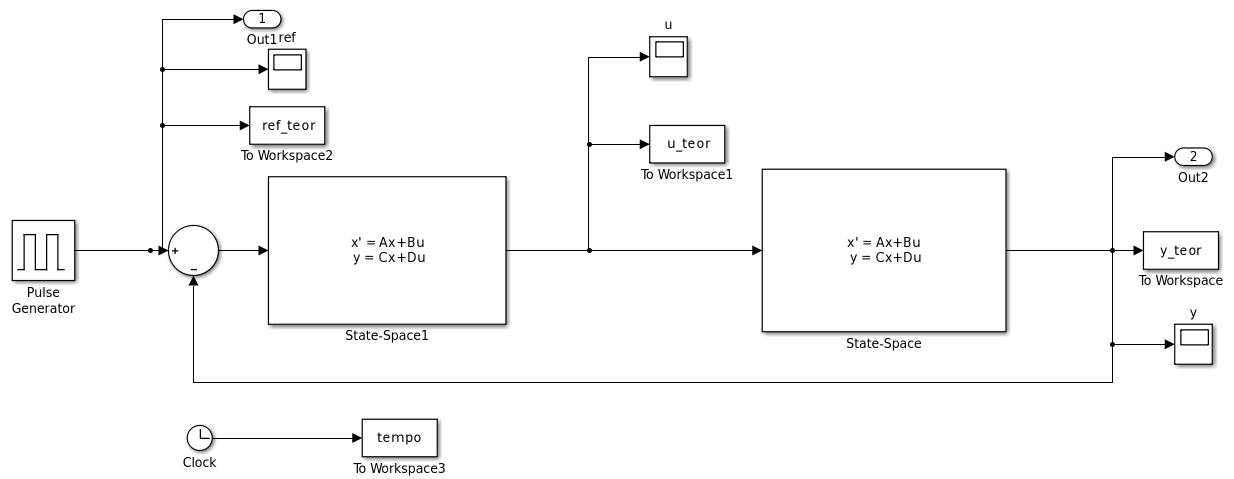
\includegraphics[width=.6\textheight]{../img/simulink.png}% Imports eps image
  \caption{\label{../img/simulink.png} Diagrama da simulação efectuada em {\it simulink}}
\end{figure*}

\fig{../img/y.png}{Saída do sistema simulado}
\fig{../img/u.png}{Estímulo do sistema simulado}

Os resultados da simulação apresentam-se nos gráficos das figuras \ref{../img/y.png} e \ref{../img/u.png} para os quais a referência é uma onda quadrada de amplitude unitária.

\section{Função de transferência em cadeira fechada}
%Determinou-se o diagrama de Bode do sistema em cadeia fechada. 
A união entre o modelo em cadeia aberta e o estimador que irão formar o sistema em cadeia fechada é realizada pela função ligacao, que recebe as matrizes do sistema em malha aberta e do estimador em malha aberta e retorna uma variável em formato sys que descreve o sistema (representado em espaço de de estados) como representado no esquema de simulink.

\fig{../img/BodeMalhaFechada.png}{Diagrama de Bode do sistema em cadeira fechada}

\section{Ensaio com o sistema real}
Foram introduzidos no real-time workshop do MATLAB os vectores de ganho obtidos para o observador assimptótico e para o controlador, e observou-se a resposta do sistema real (a barra cujo ângulo $\theta$ é medido através do potenciómetro e o ângulo de $\alpha$ é medido através do extensómetro). Apresentam-se nas figuras \ref{fig:y_t} e \ref{fig:y_d} os dados obtidos para y na simulação e com o sistema real respectivamente e nas figuras \ref{fig:u_t} e \ref{fig:u_d} os dados obtidos para u na simulação e no sistema real respectivamente:
\begin{figure}
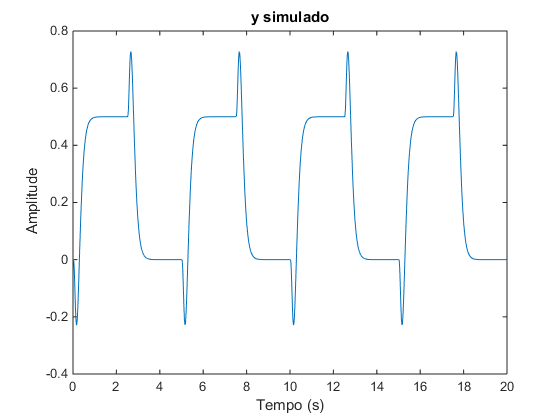
\includegraphics[width=3.5in]{../img/y.png}
\caption{Dados obtidos por Simulink para a variação da saída $(y(t))$ com o tempo}
\label{fig:y_t}
\end{figure}
\begin{figure}
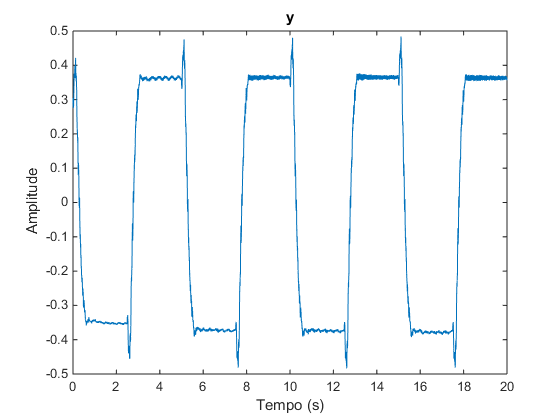
\includegraphics[width=3.5in]{../img/y_dados_01.png}
\caption{Dados obtidos para a saída ($y(t)=\theta(t)+\alpha(t)$) com o sistema real.}
\label{fig:y_d}
\end{figure}
\begin{figure}
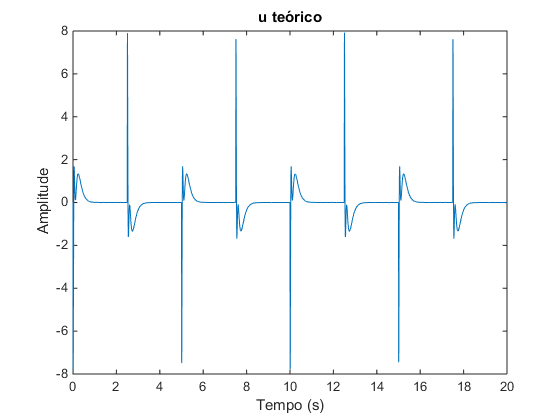
\includegraphics[width=3.5in]{../img/u.png}
\caption{Dados obtidos por Simulink para a variação da saída $(u(t))$ com o tempo}
\label{fig:u_t}
\end{figure}
\begin{figure}
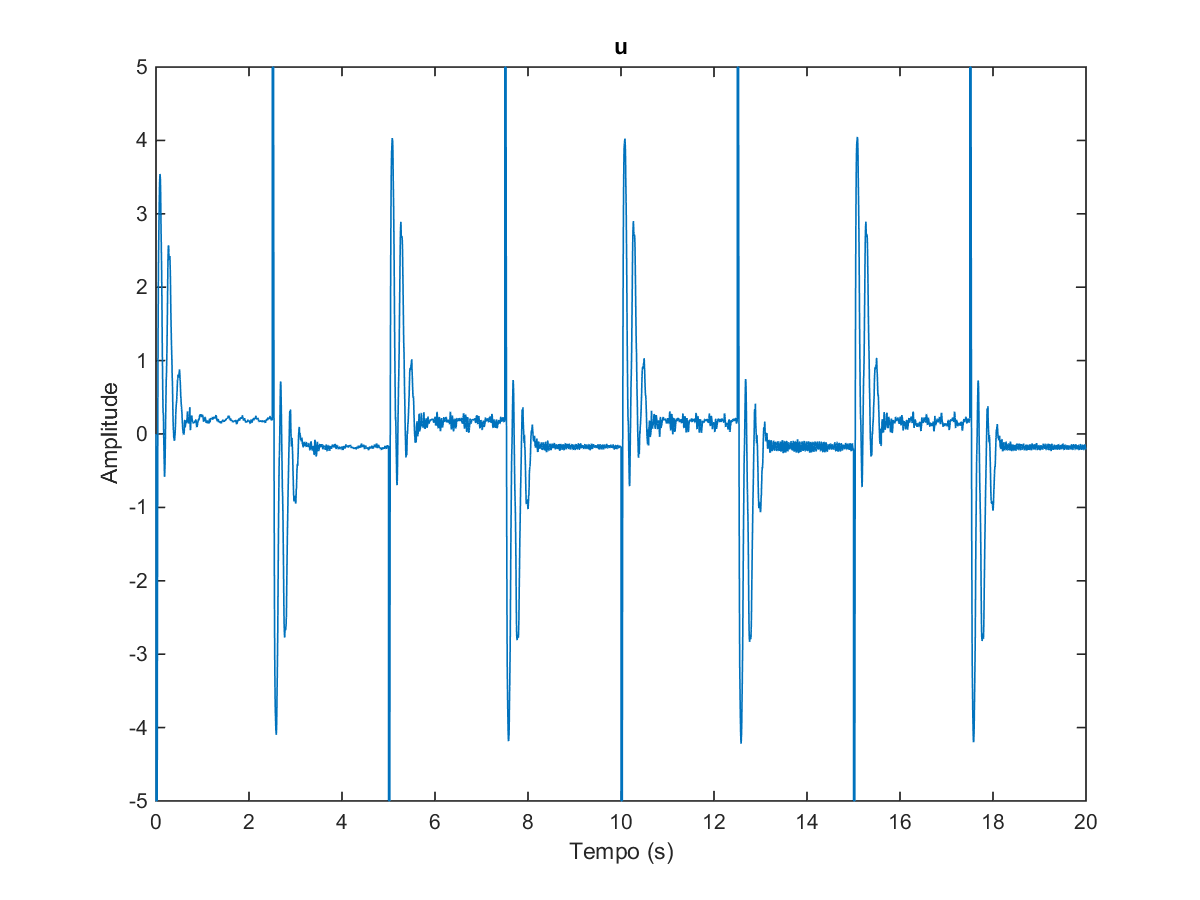
\includegraphics[width=3.5in]{../img/u_dados_01.png}
\caption{Dados obtidos para $u(t)$ com o sistema real}
\label{fig:u_d}
\end{figure}
Quanto à saída obitda é observas-se que, apesar de ser muito semelhante à saída obtida através da simulação computacional, na simulação o valor de y tende para valores bem determinados de amplitude sempre que se varia a referência (neste caso, a referência é uma onda quadrada com um período de $T=5$s), enquanto que no sistema real é possivel notar a existência de uma pequena oscilação em torno dos valores onde a barra se deveria encontrar estática. Tal siginfica que quando a barra deveria estar parada, a sua ponta ainda vibra, mesmo que pouco. Tal pode dever-se à zona morta do motor utilizado, visto que o controlador já não consegue fornecer energia suficiente para que o motor actue na barra de modo a esta ficar perfeitamente imóvel.\\
Também comparando os resultados obtidos para u, é possível confirmar a perturbação da zona morta do motor visto que o valor de u, que é o sinal que actua sobre o motor,  na simulação tende para 0 suavemente, enquanto que na prática u é uma varia impulsivamente, o que é uma tentativa do controlador de conseguir controlar o motor fora da sua zona morta. Quando o valor obtido para a ponta da barra finalmente se aproxima à com o valor na referência, o controlador continua a enviar um sinal ao motor para que este actue de modo a anular as vibrações na barra, no entanto como este não respondeo controlador continua a enviar um  sinal u diferente de 0 para actuar o motor, como se vê na figura \ref{fig:u_d}, enquanto que para um motor perfeito, como é o caso da figura \ref{fig:u_t}, o sinal u vai tender para assimptóticamente para 0.
\section{Resposta sem filtro na saída}

\section{Efeito da variação do polo do pré-filtro}

\section{Ensaio sem sinal do extensómetro}

\section{Ensaios com outras especificações para os pólos do observador e/ou controlador}

\section{Conclusões e Críticas}
\label{s:conclu}
%Incluir melhorias propostas à experiência

%\begin{acknowledgments}
%\end{acknowledgments}

%%%%%%%%%%%%%%%%%%%%%%%%%%%%%%%%%%%%%%%%%%%%%%%%%%%%%%%%%%%%%%%%%%%%%%%%%%%%%%%%
% % % % % % % % % % % % % % % %     FIM    % % % % % % % % % % % % % % % % % % % 
%%%%%%%%%%%%%%%%%%%%%%%%%%%%%%%%%%%%%%%%%%%%%%%%%%%%%%%%%%%%%%%%%%%%%%%%%%%%%%%%

\nocite{}
\bibliography{bibliografia}{}
\bibliographystyle{plain}% Produces the bibliography via BibTeX.
\end{document}
%end of file
